\documentclass{article}
\usepackage{graphicx} % Required for inserting images
\usepackage{amsmath} % For \text command
\usepackage{float}
\usepackage{graphicx} % <-- nel preambolo
\usepackage{amssymb}
\usepackage{caption}


\title{Data Mining}
\author{Clarissa Pia Rizzello}
\date{April 2025}

\begin{document}

\maketitle
\newpage
\tableofcontents
\newpage


\section{Pattern Mining}

\subsection{Data Preparation}

The \textbf{data preparation} phase for pattern mining was carried out with the aim of selecting and processing only the most semantically relevant features, in order to extract interpretable patterns.

Following an initial exploratory inspection, variables considered uninformative or redundant for the analysis—such as \texttt{originalTitle}, \texttt{totalImages}, \texttt{totalVideos}, \texttt{totalCredits}, and \texttt{canHaveEpisodes}—were removed. Additionally, the \texttt{short} label from the \texttt{titleType} feature was discarded, as this information was already represented in the \texttt{genres} attribute.

\paragraph{Categorical feature processing.}
To reduce the cardinality and asymmetry of the \texttt{countryOfOrigin} feature, a new variable \texttt{continent} was introduced via ISO mapping using the \texttt{pycountry} library. Countries that could not be mapped to a known continent (tagged as \texttt{Unknown}) were excluded to ensure semantic consistency.  
The \texttt{continent} and \texttt{genres} features, being multi-label in nature, were transformed into binary format using the \texttt{MultiLabelBinarizer} class, generating a set of binary columns with coherent prefixes (e.g., \texttt{genre\_Comedy}, \texttt{continent\_Europe}).  
The \texttt{titleType} feature was instead encoded using \texttt{get\_dummies}, producing a standard one-hot representation.

\paragraph{Transformation of numerical variables.}
A mixed approach was adopted for the numerical features, based on discretization techniques guided by empirical distributions and clustering.

The \texttt{num\_ratings} variable, which was highly skewed, was transformed using a logarithmic function (\texttt{log1p}) and subsequently standardized via \texttt{MinMaxScaler}. It was then discretized using \texttt{KMeans} clustering (\texttt{k=5}). The resulting clusters were ordered based on the median and renamed according to rating volume (\texttt{Very Low} -- \texttt{Very High}).

\begin{figure}[H]
    \centering
    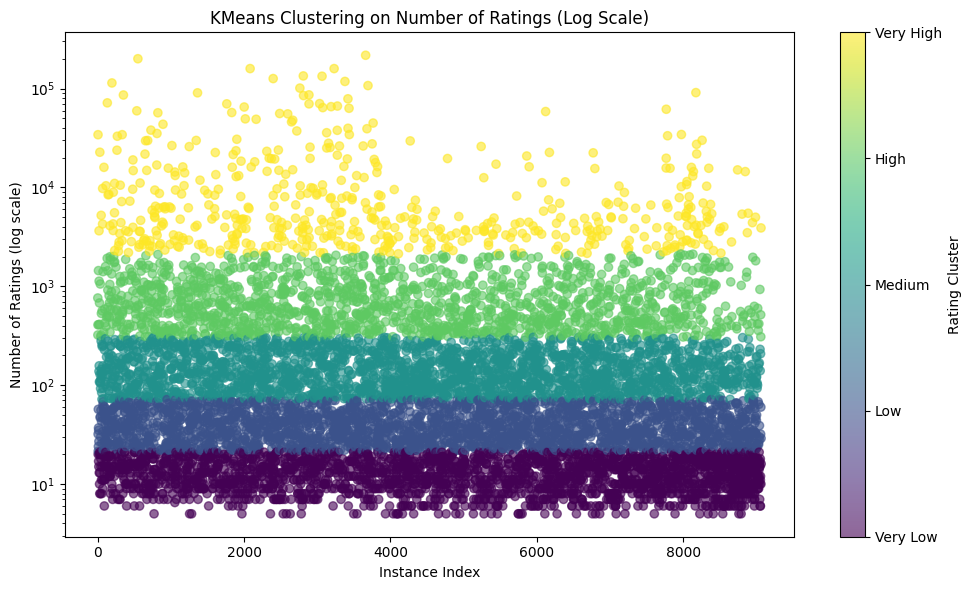
\includegraphics[width=0.5\linewidth]{Kmeans_num_rating.png}
    \caption{Scatterplot K-Means num\_ratings}
    \label{fig:enter-label}
\end{figure}


\paragraph{Definition of the \texttt{success\_class} variable.}

Since the dataset did not contain a direct measure of critical recognition, the target variable \texttt{success\_class} was constructed using a rule-based logic that incorporates both critical reviews and award-related information. In particular:
\begin{itemize}
  \item A title is labeled as \texttt{Critically Acclaimed} if it has received at least one award or one nomination;
  \item If it has not received awards or nominations but has at least one critical review, it is labeled as \texttt{Considered by Critics};
  \item Titles with no critical reviews and no recognition are classified as \texttt{Flop}.
\end{itemize}

\begin{table}[H]
    \centering
    \begin{tabular}{cc}
        Flop & 5022\\
        \hline
        Considered by Critics & 2466 \\
        \hline
        Critically Acclaimed & 1580\\
    \end{tabular}
    \caption{Distribution of the \texttt{success\_class} target variable in the development set based on critical reviews, awards, and nominations.}

    \label{tab:my_label}
\end{table}

\paragraph{Logical discretization of additional features.}
To improve the interpretability of the patterns, additional numerical variables were discretized using manually defined thresholds based on empirical criteria:

\begin{itemize}
  \item \texttt{numRegions}: \texttt{Local} if equal to 1, \texttt{Limited} if $\leq$5, \texttt{Moderate} if $\leq$10, and \texttt{International} otherwise;
  \item \texttt{rating}: \texttt{Poor} (0--5), \texttt{Average} (5--6.5), \texttt{Good} (6.5--7.5), \texttt{Excellent} ($>$7.5);
\item \texttt{runtimeMinutes}: discretized into \texttt{Short} ($\leq$60 min), \texttt{Standard} (61–90 min), \texttt{Long} (91–120 min), \texttt{Extended} (121–150 min), and \texttt{Epic} ($>$150 min) based on fixed duration intervals.

\end{itemize}



\subsection{Frequent Pattern Extraction}
The \textit{Apriori} and \textit{FP-Growth} algorithms were employed with varying values of minimum support (\texttt{min\_support}) and minimum itemset cardinality (\texttt{zmin}). The trend in the number of frequent, maximal, and closed itemsets was analyzed as a function of support thresholds, highlighting the exponential growth in the number of patterns with increasing granularity.
\subsubsection{Discussion on Frequent Patterns}

The analysis was conducted on a transactional dataset obtained by transforming the categorical and binary variables of the original dataset, representing each movie as a distinct set of items.

For each parameter combination, the following were generated:
\begin{itemize}
    \item \textbf{Maximal itemsets} (\texttt{target='m'}), which cannot be further extended without reducing support;
    \item \textbf{Closed itemsets} (\texttt{target='c'}), which preserve the maximum amount of information while reducing redundancy.
\end{itemize}

The visualizations obtained reveal that the most frequent patterns are dominated by combinations of film genres, confirming the presence of well-established semantic structures within the dataset.

\begin{figure}[H]
\centering
\begin{minipage}{0.48\textwidth}
  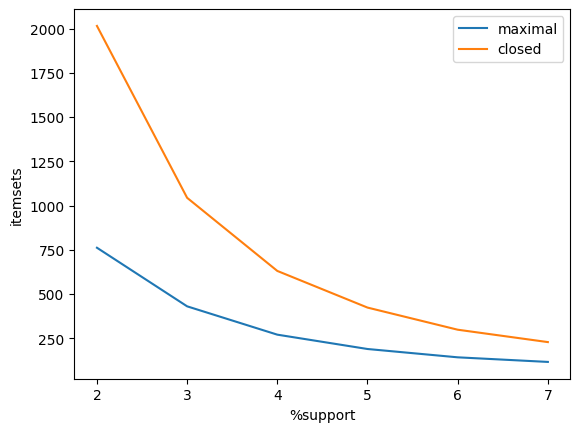
\includegraphics[width=\linewidth]{zmin2.png}
  \caption{Closed and maximal itemsets for \texttt{zmin=2}.}
  \label{fig:itemset_zmin2}
\end{minipage}
\hfill
\begin{minipage}{0.48\textwidth}
  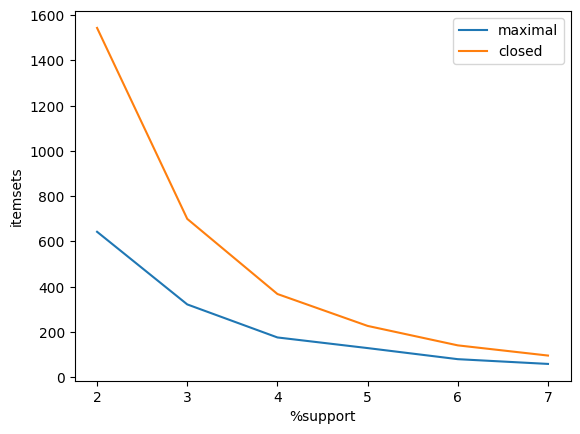
\includegraphics[width=\linewidth]{zmin3.png}
  \caption{Closed and maximal itemsets for \texttt{zmin=3}.}
  \label{fig:itemset_zmin3}
\end{minipage}
\end{figure}

As expected, increasing the support threshold leads to a significant reduction in the number of patterns. Moreover, closed itemsets consistently outnumber maximal ones, as they retain more statistical information. Raising \texttt{zmin} from 2 to 3 further decreases the number of patterns, enhancing readability at the cost of simpler pattern loss.

To compare the efficiency and productivity of the Apriori and FP-Growth algorithms, the number of itemsets generated was evaluated at different support levels and itemset sizes. The results are summarized in Table~\ref{tab:algo_comparison}.

\begin{table}[H]
\centering
\caption{Comparison between Apriori and FP-Growth across support and itemset sizes}
\label{tab:algo_comparison}
\begin{tabular}{|c|c|c|c|}
\hline
\textbf{Support (\%)} & \textbf{Itemset size} & \textbf{Apriori} & \textbf{FP-Growth} \\
\hline
8 & 2 & 170 & 113 \\
20 & 2 & 15 & 399 \\
8 & 3 & 3 & 1896 \\
20 & 3 & 64 & 176 \\
\hline
\end{tabular}
\end{table}

As observed, FP-Growth generates a significantly higher number of complex patterns (3-itemsets), particularly at lower support levels. This indicates a greater ability to explore intricate combinations, uncovering latent structures that Apriori tends to miss. In contrast, Apriori proves more efficient in detecting shorter patterns but lacks depth.

In light of these findings, FP-Growth with 8\% support and \texttt{zmin=3} was selected, as it provides an optimal balance between pattern granularity and semantic coverage, demonstrating superiority in both quantitative and qualitative terms for the purposes of this analysis.


\subsection{Association Rules Extraction}
Association rules were extracted using the FP-Growth algorithm, aimed at generating rules of the form:

\[
\text{Antecedent} \Rightarrow \text{Consequent}
\]

The rules were evaluated using three main metrics:
\begin{itemize}
  \item \textbf{Support}: the absolute or relative frequency of the rule's occurrence in the dataset;
  \item \textbf{Confidence}: the conditional probability of the consequent given the antecedent;
  \item \textbf{Lift}: the ratio between the observed confidence and the expected confidence under statistical independence.
\end{itemize}

The rules listed in Table~\ref{tab:regole_lift_alto} represent some of the most relevant patterns identified during the analysis, selected based on particularly high \textit{lift} values (greater than 2.5), indicating a strong and non-random association between antecedent and consequent.

For instance, the first rule shows that movies distributed internationally and labeled as \texttt{type\_movie} have a substantially higher likelihood of receiving a very high number of user ratings. This implies a strong relationship between distribution reach and popularity in terms of visibility and audience approval.

Another pattern highlights that internationally distributed \texttt{type\_movie} titles are often also labeled as \texttt{Critically Acclaimed}, meaning they receive positive recognition from critics. Such rules are especially relevant for predictive tasks involving the qualitative success of titles.

Various confidence thresholds were tested: with \texttt{conf = 30}, a total of 1072 rules were generated; with \texttt{conf = 40}, the number dropped to 580; and with \texttt{conf = 70}, only 101 rules remained. A threshold of \texttt{conf = 40} was ultimately selected, as it offered a good balance between quantity, semantic diversity, and rule quality. This threshold yields a manageable set of rules while maintaining sufficiently high confidence levels and often achieving lift values above 1.5, indicative of meaningful, non-trivial associations.

In fact, support, confidence, and lift were jointly analyzed to assess rule quality. Rules with high support ensure statistical robustness, while high confidence reflects strong predictive capability. However, it is the \textit{lift} that reveals the true associative strength: values significantly above 1 indicate non-random co-occurrence. For example, the rule \texttt{success\_class=Critically Acclaimed} $\Leftarrow$ \texttt{region\_distribution=International, type\_movie} presents a lift of 2.86 and a confidence of 0.50, suggesting a strong informative link between international distribution and critical recognition.

\begin{table}[H]
\centering
\caption{Examples of association rules with confidence $\geq$ 0.65 and relevant support}
\label{tab:regole_flop}
\begin{tabular}{|p{4cm}|p{5.5cm}|c|c|c|}
\hline
\textbf{Consequent} & \textbf{Antecedent} & \textbf{Conf.} & \textbf{Lift} & \textbf{Support (\%)} \\
\hline
success\_class=Flop & continent\_North America, region\_distribution=Local & 0.689 & 1.24 & 21.55 \\
\hline
region\_distribution=Local & continent\_North America, success\_class=Flop & 0.787 & 1.47 & 21.55 \\
\hline
success\_class=Flop & rating\_category=Average, region\_distribution=Local & 0.749 & 1.35 & 13.52 \\
\hline
success\_class=Flop & genre\_Drama, region\_distribution=Local & 0.655 & 1.18 & 12.26 \\
\hline
region\_distribution=Local & genre\_Drama, continent\_North America, success\_class=Flop & 0.743 & 1.39 & 6.15 \\
\hline
success\_class=Flop & rating\_category=Average, continent\_North America, region\_distribution=Local & 0.721 & 1.30 & 6.89 \\
\hline
\end{tabular}
\end{table}

\subsubsection{Discussion on Association Rules}

A relatively low confidence threshold (\texttt{$\geqslant$0.2}) was adopted to account for the strong class imbalance, as outlined in the \emph{data preparation} section. This trade-off allowed for the inclusion of rules that are predictively useful even for minority classes.

\begin{figure}[H]
\centering
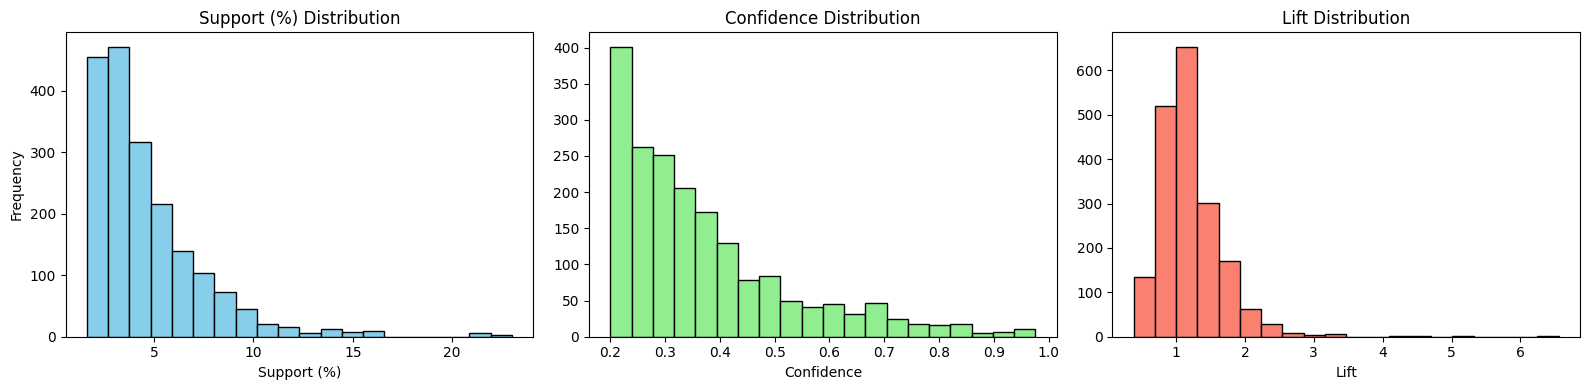
\includegraphics[width=\textwidth]{dist_sup_lift_conf.png}
\caption{Distribution of association rule metrics: support, confidence, and lift}
\label{fig:metriche_regole}
\end{figure}

Figure~\ref{fig:metriche_regole} illustrates the distributions of key metrics for the association rules extracted using the FP-Growth algorithm.

\textbf{On the left}, the support distribution confirms that most rules exhibit support between 2\% and 6\%, with a steep drop beyond this range. This behavior reflects the sparse nature of the dataset, where only a few item combinations occur frequently. Rules with support above 10\% are particularly rare.

\textbf{In the center}, the confidence distribution shows a sharply decreasing trend. The majority of rules fall within the 0.2 to 0.5 confidence range, while only a minority exceed 0.7. This implies that, while many rules are statistically valid, few demonstrate strong conditional reliability.

\textbf{On the right}, the lift distribution is concentrated around 1.0, which signals statistical independence between antecedent and consequent. However, it is noteworthy that a non-negligible number of rules achieve lift values above 1.5 and even beyond 3.0, representing highly significant co-occurrences and potentially very useful rules for descriptive or predictive purposes.

Overall, these distributions confirm that the FP-Growth algorithm was capable of identifying a diverse set of rules, many of which are statistically meaningful, albeit not always highly reliable. The high number of rules with moderate confidence but lift values above 1 suggests the presence of interesting patterns, though sometimes only partially strong or ambiguous. In supervised applications, this necessitates careful rule selection (e.g., based on lift and coverage) to prevent excessive noise in predictive models.

Subsequently, our analysis focused on extracting association rules where the target classes \texttt{success\_class} and \texttt{rating\_category} serve as consequents, in order to explore the relationship between critical reception and audience evaluation.

\begin{itemize}
    \item \textbf{success\_class} captures the level of critical acclaim, inferred from reviews, awards, and nominations;
    \item \textbf{rating\_category} reflects audience appreciation as measured by numerical ratings.
\end{itemize}

For both target variables, rules with confidence $\geq 0.2$ and lift $\geq 1.2$ were selected to ensure a meaningful balance between reliability and statistical significance.

For the class \texttt{success\_class=Flop}, several strong rules emerged:
\begin{itemize}
    \item \texttt{(rating\_category=Average, region\_distribution=Local)} $\Rightarrow$ \texttt{success\_class=Flop}, with confidence $\approx 0.75$ and lift $\approx 1.35$;
    \item \texttt{(type\_tvEpisode, continent\_North America, region\_distribution=Local)} $\Rightarrow$ \texttt{success\_class=Flop}, with confidence $\approx 0.76$ and lift $\approx 1.42$.
\end{itemize}

Similarly, highly informative rules for \texttt{success\_class=Critically Acclaimed} include:
\begin{itemize}
    \item \texttt{(region\_distribution=International, type\_movie)} $\Rightarrow$ \texttt{success\_class=Critically Acclaimed}, with confidence $\approx 0.50$ and lift $\approx 2.86$;
    \item \texttt{(genre\_Drama, type\_movie)} $\Rightarrow$ \texttt{success\_class=Critically Acclaimed}, with confidence $\approx 0.32$ and lift $\approx 1.49$.
\end{itemize}

Regarding audience perception, predictive rules for \texttt{rating\_category} were also examined. For the class \texttt{rating\_category=Good}, coherent co-occurrences emerged, such as:
\begin{itemize}
    \item \texttt{(type\_tvEpisode, continent\_North America, region\_distribution=Local)} $\Rightarrow$ \texttt{rating\_category=Good}, with confidence $\approx 0.55$ and lift $\approx 1.57$;
    \item \texttt{(type\_tvEpisode, region\_distribution=Local)} $\Rightarrow$ \texttt{rating\_category=Good}, with confidence $\approx 0.48$ and lift $\approx 1.53$.
\end{itemize}

In general, these rules show that certain content segments—such as North American local TV series—tend to be well-received by the public but may simultaneously be overlooked by critics (e.g., rules associated with \texttt{Flop}).

This dichotomy between public perception and critical evaluation is further reinforced by rules related to the class \texttt{Considered by Critics}, which display lift values above 1.6 in association with internationally distributed films of moderate popularity (\texttt{rating\_cluster=Medium} or \texttt{High N. Ratings}), albeit with lower confidence compared to rules for the \texttt{Flop} class.


\subsubsection{Application on the Test Set}

The strongest rules were subsequently applied to the test set by checking whether the rule \textit{antecedents} were fully contained within the transactions. The outcome was positive: \textbf{98\% of the transactions} in the test set triggered at least one rule, with an \textbf{average of 14.5 applicable rules per transaction}.

We analyzed the \textit{top-5} most frequently triggered rules. Some of these, although statistically strong, proved semantically trivial (e.g., \texttt{runtime\_category=Short} $\leftrightarrow$ \texttt{type\_tvEpisode}). Therefore, the focus was shifted to rules with informative \textit{consequents}, such as \texttt{success\_class} and \texttt{rating\_category}.

\begin{table}[htbp]
\centering
\caption{Association rules with \texttt{success\_class} as antecedent or consequent}
\label{tab:flop_rules}
\begin{tabular}{|p{5cm}|p{4.5cm}|c|c|c|}
\hline
\textbf{Antecedent} & \textbf{Consequent} & \textbf{Confidence} & \textbf{Lift} \\
\hline
success\_class=Flop & type\_tvEpisode & 0.461 & 1.310  \\
\hline
success\_class=Flop & region\_distribution=Local & 0.691 & 1.289 \\
\hline
region\_distribution=Local & success\_class=Flop & 0.714 & 1.289  \\
\hline
region\_distribution=Local & type\_tvEpisode & 0.598 & 1.700  \\
\hline
continent\_North America & type\_tvEpisode & 0.444 & 1.261 \\
\hline
\end{tabular}
\end{table}

\begin{table}[htbp]
\centering
\caption{Predictive rules for the \texttt{rating\_category} class}
\label{tab:rating_good_rules}
\begin{tabular}{|p{6.5cm}|p{3.5cm}|c|c|}
\hline
\textbf{Antecedent} & \textbf{Consequent} & \textbf{Conf.} & \textbf{Lift} \\
\hline
type\_tvEpisode, continent\_North America, region\_distribution=Local & rating\_category=Good & 0.508 & 1.634 \\
\hline
type\_tvEpisode, continent\_North America & rating\_category=Good & 0.506 & 1.629 \\
\hline
type\_tvEpisode, region\_distribution=Local & rating\_category=Good & 0.492 & 1.583 \\
\hline
type\_tvEpisode & rating\_category=Good & 0.485 & 1.561 \\
\hline
type\_tvEpisode, \newline region\_distribution=Local, \newline success\_class=Flop & rating\_category=Good & 0.479 & 1.543 \\
\hline
\end{tabular}
\end{table}

This demonstrates how the identified rules are applied to the test set, showing that they are particularly effective for predicting the majority classes such as \texttt{Flop} for \texttt{success\_class} and \texttt{Good} for \texttt{rating\_category}.


\subsection{Predictive Use of the Rules}
The extracted rules were employed to construct a rule-based classifier, where the prediction for each instance is obtained by selecting, among the applicable rules (i.e., those whose antecedents are contained in the transaction), the one with the highest confidence.

\textbf{For the variable \texttt{success\_class}}, the classifier achieved an accuracy of 67.8\%, with particularly strong performance on the \texttt{Flop} class (precision 0.74, recall 0.93, F1-score 0.82). This result reflects the abundance of high-confidence and high-support rules associated with this category. In contrast, the \texttt{Critically Acclaimed} and \texttt{Considered by Critics} classes were predicted with low accuracy, especially in terms of recall (0.18 and 0.35 respectively), indicating reduced predictive coverage for these categories.

\textbf{For the variable \texttt{rating\_category}}, the overall accuracy was approximately 49\%. The only classes effectively predicted were \texttt{Average} (F1-score 0.61) and \texttt{Good} (F1-score 0.51), while \texttt{Excellent} and \texttt{Poor} were never predicted by the model (recall 0.00), due to the absence of sufficiently strong rules associated with these classes. This significantly limits the model's generalizability and confirms the impact of class imbalance in the dataset.

In addition to accuracy, precision, recall, and F1-score were evaluated, highlighting how the rule-based approach tends to favor majority classes while neglecting less represented ones. The predictive power of the classifier is thus highly asymmetric, a direct consequence of the greater availability of frequent and reliable rules for dominant classes.

In summary, while the rule-based system performs well for the most common classes, its effectiveness drops considerably when it comes to covering minority classes. This reveals a structural limitation of the approach, which relies on the empirical frequency of itemsets and therefore struggles to generate reliable predictions in the presence of highly imbalanced class distributions.

\section{Conclusions}

The analysis conducted has demonstrated the effectiveness of pattern mining in extracting interpretable knowledge from complex data within the film domain. Following a thorough phase of data preparation and transformation, the application of both FP-Growth and Apriori algorithms enabled the identification of frequent patterns and association rules characterized by substantial levels of support, confidence, and lift.

The FP-Growth algorithm proved preferable due to its ability to generate a significantly higher number of informative rules, particularly for larger itemsets, while maintaining efficient computational performance.

The derived rules highlighted meaningful relationships between movie features, geographical distribution, genres, and success metrics (both critical and audience-based). In particular, a clear distinction emerged between patterns associated with critical acclaim and those related to audience ratings, underlining the utility of this approach for comparative and predictive analysis.

The rule-based classification system produced mixed results. For the variable \texttt{success\_class}, the model achieved a notable accuracy of 67.8\%, showing strong performance for the majority class \texttt{Flop}. However, predictive performance was limited for minority classes. A similar trend was observed for \texttt{rating\_category}, with an overall accuracy of 49% and poor coverage of the \texttt{Excellent} and \texttt{Poor} categories.

In summary, the rule-based approach demonstrated good descriptive and interpretative potential but exhibited clear limitations in imbalanced supervised learning contexts. The reliance on empirical itemset frequency poses a structural constraint, making it difficult to produce reliable predictions for underrepresented classes.

Future enhancements may include:
\begin{itemize}
\item the adoption of class balancing techniques (e.g., oversampling or synthetic rule generation);
\item integration with hybrid models combining rules and machine learning classifiers;
\item automatic rule selection based on multi-objective criteria such as coverage, confidence, and lift.
\end{itemize}

Overall, the pattern mining process, when appropriately tuned, remains a powerful and flexible tool for data exploration, classification, and semantic enrichment.


\end{document}
